% This LaTeX document needs to be compiled with XeLaTeX.
\documentclass[10pt]{article}
\usepackage[utf8]{inputenc}
\usepackage{graphicx}
\usepackage[export]{adjustbox}
\graphicspath{ {./images/} }
\usepackage{amsmath}
\usepackage{amsfonts}
\usepackage{amssymb}
\usepackage[version=4]{mhchem}
\usepackage{stmaryrd}
\usepackage[fallback]{xeCJK}
\usepackage{polyglossia}
\usepackage{fontspec}
\setCJKmainfont{Noto Serif CJK TC}

\setmainlanguage{polish}
\setmainfont{CMU Serif}

\title{ARKUSZ PRÓBNEJ MATURY Z OPERONEM MATEMATYKA }

\author{}
\date{}


\begin{document}
\maketitle
\section*{POZIOM PODSTAWOWY}
\section*{Czas pracy: 170 minut}
\section*{Instrukcja dla zdającego}
\begin{enumerate}
  \item Sprawdź, czy arkusz egzaminacyjny zawiera 14 stron (zadania 1.-32.). Ewentualny brak zgłoś przewodniczącemu zespołu nadzorującego egzamin.
  \item Rozwiązania zadań i odpowiedzi zapisz w miejscu na to przeznaczonym.
  \item W zadaniach zamkniętych (1.-23.) zaznacz jedną poprawną odpowiedź.
  \item W rozwiązaniach zadań otwartych (24.-32.) przedstaw tok rozumowania prowadzący do ostatecznego wyniku.
  \item Pisz czytelnie. Używaj długopisu/pióra tylko z czarnym tuszem/atramentem.
  \item Nie używaj korektora, a błędne zapisy wyraźnie przekreśl.
  \item Zapisy w brudnopisie nie będą oceniane.
  \item Obok numeru każdego zadania podana jest maksymalna liczba punktów możliwych do uzyskania.
  \item Możesz korzystać z zestawu wzorów matematycznych, cyrkla i linijki oraz kalkulatora.
\end{enumerate}

\section*{Życzymy powodzenia!}
Za rozwiązanie wszystkich zadań można otrzymać łącznie 50 punktów.\\

\includegraphics[max width=\textwidth, center]{2024_11_21_f15c19552e6d78b9dfffg-01}

KOD ZDAJĄCEGO

PESEL ZDAJĄCEGO

LISTOPAD\\
2017

Wpisuje zdający przed rozpoczęciem pracy\\
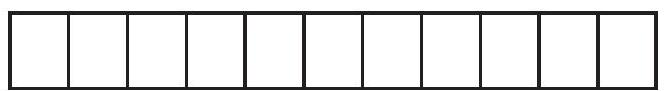
\includegraphics[max width=\textwidth, center]{2024_11_21_f15c19552e6d78b9dfffg-01(1)}

\section*{ZADANIA ZAMKNIETE}
W zadaniach 1.-23. wybierz i zaznacz jedną poprawną odpowiedź.

\section*{Zadanie 1. (0-1)}
Liczba \(\log _{2} \frac{1}{\sqrt{8}}\) jest równa:\\
A. \(-\frac{3}{2}\)\\
B. \(\frac{3}{2}\)\\
C. \(\frac{1}{3}\)\\
D. \(-\frac{1}{3}\)

Zadanie 2. (0-1)\\
Liczba \(a=\frac{14 \sqrt{2}}{\sqrt{2}-3}\) należy do przedziału:\\
A. \((-\infty,-13)\)\\
B. \(\langle-13,-12)\)\\
C. \((12,13\rangle\)\\
D. \((13,+\infty)\)

\section*{Zadanie 3. (0-1)}
Reszta z dzielenia liczby naturalnej \(x\) przez 9 jest równa 7. Reszta z dzielenia kwadratu tej liczby przez 9 jest równa:\\
A. 2\\
B. 4\\
C. 6\\
D. 8

\section*{Zadanie 4. (0-1)}
Prosta \(l\) przechodzi przez punkty \(A=(6,-7), B=(-10,3)\). Prosta \(k\) jest symetralną odcinka \(A B\). Współczynnik kierunkowy prostej \(k\) jest równy:\\
A. \(-\frac{8}{5}\)\\
B. \(\frac{8}{5}\)\\
C. \(\frac{5}{8}\)\\
D. \(-\frac{5}{8}\)

Zadanie 5. (0-1)\\
Dany jest ciąg \(\left(a_{n}\right)\) o wyrazie ogólnym \(a_{n}=\frac{2 n+1}{n+3}\). Liczby \(a_{3}, a_{5}\) są wyrazami tego ciągu, a liczby \(\left(a_{3}, x, a_{5}\right)\) tworzą ciąg arytmetyczny. Liczba \(x\) jest równa:\\
A. \(x=\frac{61}{48}\)\\
B. \(x=\frac{61}{96}\)\\
C. \(x=\frac{69}{96}\)\\
D. \(x=\frac{69}{48}\)

\section*{Zadanie 6. (0-1)}
Dana jest funkcja określona wzorem \(y=x^{2}-4 \sqrt{3} x+12\). Trzecia potęga jedynego miejsca zerowego tej funkcji to liczba:\\
A. \(8 \sqrt{3}\)\\
B. 24\\
C. \(24 \sqrt{3}\)\\
D. 12

\section*{Zadanie 7. (0-1)}
Do wykresu funkcji wykładniczej \(f(x)=\left(\frac{1}{4}\right)^{x}\) należy punkt:\\
A. \(A=\left(-\frac{1}{2},-2\right)\)\\
B. \(A=\left(-\frac{1}{2}, 2\right)\)\\
C. \(A=\left(2, \frac{1}{2}\right)\)\\
D. \(A=\left(2,-\frac{1}{2}\right)\)

BRUDNOPIS (nie podlega ocenie)\\

\includegraphics[max width=\textwidth, center]{2024_11_21_f15c19552e6d78b9dfffg-03}

\section*{Zadanie 8. (0-1)}
Dany jest ciąg geometryczny o wyrazach różnych od 0 . Suma siódmego i ósmego wyrazu tego ciągu jest równa 0 . Oznacza to, że suma tysiąca początkowych wyrazów tego ciągu jest równa:\\
A. \(1000 a_{1}\)\\
B. \(1001 a_{1}\)\\
C. 10\\
D. 0

\section*{Zadanie 9. (0-1)}
Punkty \(A, B, C, D\) należą do okręgu o środku \(O\). Jeśli kąt \(A B C\) ma miarę \(70^{\circ}\), to kąt \(D A C\) ma miarę:\\
A. \(70^{\circ}\)\\
B. \(50^{\circ}\)\\
C. \(40^{\circ}\)\\
D. \(20^{\circ}\)

\section*{Zadanie 10. (0-1)}
\begin{center}
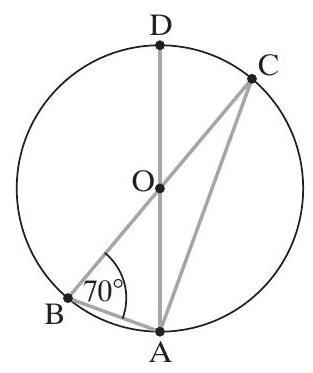
\includegraphics[max width=\textwidth]{2024_11_21_f15c19552e6d78b9dfffg-04}
\end{center}

Trójkąty \(A B C\) i \(D E F\) są podobne. Obwód trójkąta \(A B C\) jest równy 16, a jego pole 12. Pole trójkąta \(D E F\) jest równe 60 . Zatem obwód trójkąta \(D E F\) jest równy:\\
A. 80\\
B. \(16 \sqrt{5}\)\\
C. \(\frac{16 \sqrt{5}}{5}\)\\
D. \(\frac{16}{5}\)

\section*{Zadanie 11. (0-1)}
Wykres funkcji \(f(x)=(4 m-2) x+k-3\) przechodzi tylko przez II i IV ćwiartkę układu współrzędnych. Oznacza to, że:\\
A. \(\left\{\begin{array}{l}m>\frac{1}{2} \\ k=-3\end{array}\right.\)\\
B. \(\left\{\begin{array}{l}m<\frac{1}{2} \\ k=-3\end{array}\right.\)\\
C. \(\left\{\begin{array}{l}m<\frac{1}{2} \\ k=3\end{array}\right.\)\\
D. \(\left\{\begin{array}{l}m>\frac{1}{2} \\ k=3\end{array}\right.\)

Zadanie 12. (0-1)\\
Wzór funkcji, której wykres powstaje przez symetrię osiową względem osi \(O X\) wykresu funkcji \(f(x)=x^{2}-4\), to:\\
A. \(f(x)=(x+4)^{2}\)\\
B. \(f(x)=-x^{2}-4\)\\
C. \(f(x)=-x^{2}+4\)\\
D. \(f(x)=(x-4)^{2}\)

\section*{Zadanie 13. (0-1)}
Wyrażenie wymierne \(W=\frac{x-3}{x^{2}-4 x+4}\) jest określone dla\\
A. \(x \in R\)\\
B. \(x \in \backslash\{3\}\)\\
C. \(x \in R \backslash\{2\}\)\\
D. \(x \in R \backslash\{-2,2\}\)

\section*{Zadanie 14. (0-1)}
W trójkącie prostokątnym \(A B C\) przyprostokątne różnią się o 4 , a jeden z kątów ma miarę \(30^{\circ}\). Krótsza przyprostokątna tego trójkąta ma długość:\\
A. \(\frac{2 \sqrt{3}}{3}\)\\
B. \(\frac{2 \sqrt{3}}{6}\)\\
C. \(2 \sqrt{3}-2\)\\
D. \(2 \sqrt{3}+2\)

\section*{Zadanie 15. (0-1)}
Rozwiązaniem nierówności \((3 x+9)^{2}>0\) jest:\\
A. zbiór \(R\)\\
B. zbiór pusty\\
C. zbiór \(R \backslash\{-3\}\)\\
D. zbiór \(R \backslash\{-9\}\)

BRUDNOPIS (nie podlega ocenie)\\

\includegraphics[max width=\textwidth, center]{2024_11_21_f15c19552e6d78b9dfffg-05}

\section*{Zadanie 16. (0-1)}
Jeśli \(A=(-\infty, 0)\) i \(B=\langle 0,5\rangle\), to różnica przedziałów \(B\) i \(A\) jest równa:\\
A. \((-\infty, 0)\)\\
B. \((-\infty, 0\rangle\)\\
C. \((0,5\rangle\)\\
D. \(\langle 0,5\rangle\)

\section*{Zadanie 17. (0-1)}
Dany jest trójkąt \(A B C\) o bokach długości 4 i 6 . Pole tego trójkąta jest równe \(3 \sqrt{15}\). Oznacza to, że jeśli kąt między bokami o długościach 4 i 6 ma miarę \(\alpha>90^{\circ}\), to:\\
A. \(\cos \alpha=\frac{\sqrt{15}}{4}\)\\
B. \(\cos \alpha=\frac{1}{4}\)\\
C. \(\cos \alpha=-\frac{\sqrt{15}}{4}\)\\
D. \(\cos \alpha=-\frac{1}{4}\)

\section*{Zadanie 18. (0-1)}
Rzucono cztery razy monetą. Prawdopodobieństwo tego, że wypadnie co najwyżej 1 orzeł, jest równe:\\
A. \(\frac{2}{8}\)\\
B. \(\frac{5}{16}\)\\
C. \(\frac{4}{8}\)\\
D. \(\frac{4}{16}\)

Zadanie 19. (0-1)\\
Przekrój osiowy stożka jest trójkątem prostokątnym o przeciwprostokątnej długości 12. Pole powierzchni całkowitej stożka jest równe:\\
A. \(6 \pi(1+\sqrt{2})\)\\
B. \(36 \pi(1+\sqrt{2})\)\\
C. \(24 \pi\)\\
D. \(36 \pi\)

\section*{Zadanie 20. (0-1)}
Suma \(n\) początkowych wyrazów ciągu arytmetycznego wyraża się wzorem \(S_{n}=3 n^{2}+4 n\). Piąty wyraz tego ciągu jest równy:\\
A. 45\\
B. 31\\
C. 21\\
D. 11

\section*{Zadanie 21. (0-1)}
Funkcja \(f(x)=(m+3) x^{2}+16 x+5\) osiąga wartość największą dla \(x=2\). Oznacza to, że największa wartość tej funkcji jest równa:\\
A. -7\\
B. -14\\
C. 14\\
D. 21

\section*{Zadanie 22. (0-1)}
Sześcian \(A B C D A^{\prime} B^{\prime} C^{\prime} D^{\prime}\) przecięto płaszczyzną przechodzącą przez przekątną \(B D\) dolnej podstawy i wierzchołek \(C^{\prime}\) górnej podstawy. Jeśli \(a\) jest krawędzią tego sześcianu, to pole otrzymanego przekroju jest równe:\\
A. \(\frac{1}{2} a^{2} \sqrt{2}\)\\
B. \(\frac{1}{2} a^{2} \sqrt{3}\)\\
C. \(\frac{1}{2} a^{2} \sqrt{5}\)\\
D. \(\frac{1}{2} a^{2} \sqrt{6}\)

\section*{Zadanie 23. (0-1)}
Jeśli \(x+\frac{1}{x}=6\), to:\\
A. \(x^{2}+\frac{1}{x^{2}}=2 \sqrt{6}\)\\
B. \(x^{2}+\frac{1}{x^{2}}=\sqrt{6}\)\\
C. \(x^{2}+\frac{1}{x^{2}}=36\)\\
D. \(x^{2}+\frac{1}{x^{2}}=34\)

BRUDNOPIS (nie podlega ocenie)\\

\includegraphics[max width=\textwidth, center]{2024_11_21_f15c19552e6d78b9dfffg-07}

\section*{ZADANIA OTWARTE}
Rozwiązania zadań 24.-32. należy zapisać w wyznaczonych miejscach pod treścią zadania.

Zadanie 24. (0-2)\\
Rozwiąż nierówność \((4 x-1)^{2}<(2-5 x)^{2}\).\\

\includegraphics[max width=\textwidth, center]{2024_11_21_f15c19552e6d78b9dfffg-08}

Odpowiedź:

\section*{Zadanie 25. (0-2)}
Narysuj wykres funkcji \(f(x)=2^{x}-3\). Podaj zbiór wartości tej funkcji.

\begin{center}
\begin{tabular}{|c|c|c|c|c|c|c|c|c|c|c|c|c|c|c|c|c|c|c|c|c|c|c|c|c|}
\hline
 &  &  &  &  &  &  &  &  &  &  &  &  &  &  &  &  &  &  &  &  &  &  &  &  \\
\hline
 &  &  &  &  &  &  &  &  &  &  &  &  &  &  &  &  &  &  &  &  &  &  &  &  \\
\hline
 &  &  &  &  &  &  &  &  &  &  &  &  &  &  &  &  &  &  &  &  &  &  &  &  \\
\hline
 &  &  &  &  &  &  &  &  &  &  &  &  &  &  &  &  &  &  &  &  &  &  &  &  \\
\hline
 &  &  &  &  &  &  &  &  &  &  &  &  &  &  &  &  &  &  &  &  &  &  &  &  \\
\hline
 &  &  &  &  &  &  &  &  &  &  &  &  &  &  &  &  &  &  &  &  &  &  &  &  \\
\hline
 &  &  &  &  &  &  &  &  &  &  &  &  &  &  &  &  &  &  &  &  &  &  &  &  \\
\hline
 &  &  &  &  &  &  &  &  &  &  &  &  &  &  &  &  &  &  &  &  &  &  &  &  \\
\hline
 &  &  &  &  &  &  &  &  &  &  &  &  &  &  &  &  &  &  &  &  &  &  &  &  \\
\hline
 &  &  &  &  &  &  &  &  &  &  &  &  &  &  &  &  &  &  &  &  &  &  &  &  \\
\hline
 &  &  &  &  &  &  &  &  &  &  &  &  &  &  &  &  &  &  &  &  &  &  &  &  \\
\hline
 &  &  &  &  &  &  &  &  &  &  &  &  &  &  &  &  &  &  &  &  &  &  &  &  \\
\hline
 &  &  &  &  &  &  &  &  &  &  &  &  &  &  &  &  &  &  &  &  &  &  &  &  \\
\hline
 &  &  &  &  &  &  &  &  &  &  &  &  &  &  &  &  &  &  &  &  &  &  &  &  \\
\hline
 &  &  &  &  &  &  &  &  &  &  &  &  &  &  &  &  &  &  &  &  &  &  &  &  \\
\hline
\end{tabular}
\end{center}

Odpowiedź:

\section*{Zadanie 26. (0-2)}
Wykaż, że jeśli liczba rzeczywista \(a\) spełnia warunek \(a<1\), to \(\frac{1}{1-a} \geq 4 a\).

\begin{center}
\begin{tabular}{|c|c|c|c|c|c|c|c|c|c|c|c|c|c|c|c|c|c|c|c|c|c|c|}
\hline
 &  &  &  &  & 到 &  &  &  &  & - &  &  &  &  &  &  &  &  &  &  &  &  \\
\hline
 &  &  &  &  &  &  &  &  &  &  &  &  &  &  &  &  &  &  &  &  &  &  \\
\hline
 &  &  &  &  &  &  &  &  &  &  &  &  &  &  &  &  &  &  &  &  &  &  \\
\hline
 &  &  &  &  &  &  &  &  &  &  &  &  &  &  &  &  &  &  &  &  &  &  \\
\hline
 &  &  &  &  &  &  &  &  &  &  &  &  &  &  &  &  &  &  &  &  &  &  \\
\hline
 &  &  &  &  &  &  &  &  &  &  &  &  &  &  &  &  &  &  &  &  &  &  \\
\hline
 &  &  &  &  &  &  &  &  &  &  &  &  &  &  &  &  &  &  &  &  &  &  \\
\hline
 &  &  &  &  &  &  &  &  &  &  &  &  &  &  &  &  &  &  &  &  &  &  \\
\hline
 &  &  &  &  &  &  &  &  &  &  &  &  &  &  &  &  &  &  &  &  &  &  \\
\hline
 &  &  &  &  &  &  &  &  &  &  &  &  &  &  &  &  &  &  &  &  &  &  \\
\hline
 &  &  &  &  &  &  &  &  &  &  &  &  &  &  &  &  &  &  &  &  &  &  \\
\hline
 &  &  &  &  &  &  &  &  &  &  &  &  &  &  &  &  &  &  &  &  &  &  \\
\hline
 &  &  &  &  &  &  &  &  &  &  &  &  &  &  &  &  &  &  &  &  &  &  \\
\hline
 &  &  &  &  &  &  &  &  &  &  &  &  &  &  &  &  &  &  &  &  &  &  \\
\hline
 &  &  &  &  &  &  &  &  &  &  &  &  &  &  &  &  &  &  &  &  &  &  \\
\hline
\end{tabular}
\end{center}

Odpowiedź: \(\qquad\)

\section*{Zadanie 27. (0-2)}
Wyznacz współczynniki \(b, c\) we wzorze funkcji \(f(x)=x^{2}+b x+c\), jeśli wiesz, że miejsca zerowe tej funkcji są równe (-4) i 2.

\begin{center}
\begin{tabular}{|c|c|c|c|c|c|c|c|c|c|c|c|c|c|c|c|c|c|c|c|c|c|c|}
\hline
 &  &  &  &  &  &  &  &  &  &  &  &  &  &  &  &  &  &  &  &  &  &  \\
\hline
 &  &  &  &  &  &  &  &  &  &  &  &  &  &  &  &  &  &  &  &  &  &  \\
\hline
 &  &  &  &  &  &  &  &  &  &  &  &  &  &  &  &  &  &  &  &  &  &  \\
\hline
 &  &  &  &  &  &  &  &  &  &  &  &  &  &  &  &  &  &  &  &  &  &  \\
\hline
 &  &  &  &  &  &  &  &  &  &  &  &  &  &  &  &  &  &  &  &  &  &  \\
\hline
 &  &  &  &  &  &  &  &  &  &  &  &  &  &  &  &  &  &  &  &  &  &  \\
\hline
 &  &  &  &  &  &  &  &  &  &  &  &  &  &  &  &  &  &  &  &  &  &  \\
\hline
 &  &  &  &  &  &  &  &  &  &  &  &  &  &  &  &  &  &  &  &  &  &  \\
\hline
 &  &  &  &  &  &  &  &  &  &  &  &  &  &  &  &  &  &  &  &  &  &  \\
\hline
 &  &  &  &  &  &  &  &  &  &  &  &  &  &  &  &  &  &  &  &  &  &  \\
\hline
 &  &  &  &  &  &  &  &  &  &  &  &  &  &  &  &  &  &  &  &  &  &  \\
\hline
 &  &  &  &  &  &  &  &  &  &  &  &  &  &  &  &  &  &  &  &  &  &  \\
\hline
 &  &  &  &  &  &  &  &  &  &  &  &  &  &  &  &  &  &  &  &  &  &  \\
\hline
 &  &  &  &  &  &  &  &  &  &  &  &  &  &  &  &  &  &  &  &  &  &  \\
\hline
 &  &  &  &  &  &  &  &  &  &  &  &  &  &  &  &  &  &  &  &  &  &  \\
\hline
\end{tabular}
\end{center}

Odpowiedź: \(\qquad\)

\section*{Zadanie 28. (0-2)}
Wykaż, że jeśli liczby \(\left(3^{a}, 3^{b}, 3^{c}\right)\) tworzą ciąg geometryczny, to liczby \((a, b, c)\) tworzą ciąg arytmetyczny.\\

\includegraphics[max width=\textwidth, center]{2024_11_21_f15c19552e6d78b9dfffg-10}

\section*{Zadanie 29. (0-2)}
Rzucono trzy razy sześcienną kostką do gry. Oblicz prawdopodobieństwo tego, że suma wyrzuconych oczek jest równa co najmniej 16.\\

\includegraphics[max width=\textwidth, center]{2024_11_21_f15c19552e6d78b9dfffg-10(1)}

Odpowiedź:

\section*{Zadanie 30. (0-4)}
Wyznacz długość boku kwadratu wpisanego w trójkąt równoboczny o boku \(a\) w ten sposób, że jeden bok kwadratu jest zawarty w boku trójkąta, a dwa wierzchołki kwadratu należą do pozostałych boków trójkąta.

\begin{center}
\begin{tabular}{|c|c|c|c|c|c|c|c|c|c|c|c|c|c|c|c|c|c|c|c|c|c|c|}
\hline
 &  &  &  &  &  &  &  &  &  &  &  &  &  &  &  &  &  &  &  &  &  &  \\
\hline
 &  &  &  &  &  &  &  &  &  &  &  &  &  &  &  &  &  &  &  &  &  &  \\
\hline
 &  &  &  &  &  &  &  &  &  &  &  &  &  &  &  &  &  &  &  &  &  &  \\
\hline
 &  &  &  &  &  &  &  &  &  &  &  &  &  &  &  &  &  &  &  &  &  &  \\
\hline
 &  &  &  &  &  &  &  &  &  &  &  &  &  &  &  &  &  &  &  &  &  &  \\
\hline
 &  &  &  &  &  &  &  &  &  &  &  &  &  &  &  &  &  &  &  &  &  &  \\
\hline
 &  &  &  &  &  &  &  &  &  &  &  &  &  &  &  &  &  &  &  &  &  &  \\
\hline
 &  &  &  &  &  &  &  &  &  &  &  &  &  &  &  &  &  &  &  &  &  &  \\
\hline
 &  &  &  &  &  &  &  &  &  &  &  &  &  &  &  &  &  &  &  &  &  &  \\
\hline
 &  &  &  &  &  &  &  &  &  &  &  &  &  &  &  &  &  &  &  &  &  &  \\
\hline
 &  &  &  &  &  &  &  &  &  &  &  &  &  &  &  &  &  &  &  &  &  &  \\
\hline
 &  &  &  &  &  &  &  &  &  &  &  &  &  &  &  &  &  &  &  &  &  &  \\
\hline
 &  &  &  &  &  &  &  &  &  &  &  &  &  &  &  &  &  &  &  &  &  &  \\
\hline
 &  &  &  &  &  &  &  &  &  &  &  &  &  &  &  &  &  &  &  &  &  &  \\
\hline
 &  &  &  &  &  &  &  &  &  &  &  &  &  &  &  &  &  &  &  &  &  &  \\
\hline
 &  &  &  &  &  &  &  &  &  &  &  &  &  &  &  &  &  &  &  &  &  &  \\
\hline
 &  &  &  &  &  &  &  &  &  &  &  &  &  &  &  &  &  &  &  &  &  &  \\
\hline
 &  &  &  &  &  &  &  &  &  &  &  &  &  &  &  &  &  &  &  &  &  &  \\
\hline
 &  &  &  &  &  &  &  &  &  &  &  &  &  &  &  &  &  &  &  &  &  &  \\
\hline
 &  &  &  &  &  &  &  &  &  &  &  &  &  &  &  &  &  &  &  &  &  &  \\
\hline
 &  &  &  &  &  &  &  &  &  &  &  &  &  &  &  &  &  &  &  &  &  &  \\
\hline
 &  &  &  &  &  &  &  &  &  &  &  &  &  &  &  &  &  &  &  &  &  &  \\
\hline
 &  &  &  &  &  &  &  &  &  &  &  &  &  &  &  &  &  &  &  &  &  &  \\
\hline
 &  &  &  &  &  &  &  &  &  &  &  &  &  &  &  &  &  &  &  &  &  &  \\
\hline
 &  &  &  &  &  &  &  &  &  &  &  &  &  &  &  &  &  &  &  &  &  &  \\
\hline
 &  &  &  &  &  &  &  &  &  &  &  &  &  &  &  &  &  &  &  &  &  &  \\
\hline
 &  &  &  &  &  &  &  &  &  &  &  &  &  &  &  &  &  &  &  &  &  &  \\
\hline
 &  &  &  &  &  &  &  &  &  &  &  &  &  &  &  &  &  &  &  &  &  &  \\
\hline
 &  &  &  &  &  &  &  &  &  &  &  &  &  &  &  &  &  &  &  &  &  &  \\
\hline
 &  &  &  &  &  &  &  &  &  &  &  &  &  &  &  &  &  &  &  &  &  &  \\
\hline
 &  &  &  &  &  &  &  &  &  &  &  &  &  &  &  &  &  &  &  &  &  &  \\
\hline
 &  &  &  &  &  &  &  &  &  &  &  &  &  &  &  &  &  &  &  &  &  &  \\
\hline
 &  &  &  &  &  &  &  &  &  &  &  &  &  &  &  &  &  &  &  &  &  &  \\
\hline
 &  &  &  &  &  &  &  &  &  &  &  &  &  &  &  &  &  &  &  &  &  &  \\
\hline
 &  &  &  &  &  &  &  &  &  &  &  &  &  &  &  &  &  &  &  &  &  &  \\
\hline
 &  &  &  &  &  &  &  &  &  &  &  &  &  &  &  &  &  &  &  &  &  &  \\
\hline
 &  &  &  &  &  &  &  &  &  &  &  &  &  &  &  &  &  &  &  &  &  &  \\
\hline
 &  &  &  &  &  &  &  &  &  &  &  &  &  &  &  &  &  &  &  &  &  &  \\
\hline
 &  &  &  &  &  &  &  &  &  &  &  &  &  &  &  &  &  &  &  &  &  &  \\
\hline
 &  &  &  &  &  &  &  &  &  &  &  &  &  &  &  &  &  &  &  &  &  &  \\
\hline
 &  &  &  &  &  &  &  &  &  &  &  &  &  &  &  &  &  &  &  &  &  &  \\
\hline
\end{tabular}
\end{center}

Odpowiedź:

Zadanie 31. (0-5)\\
Dane są punkty \(A=(4,2)\) i \(B=(1,-3)\). Wyznacz współrzędne punktu \(C\) należącego do osi \(O Y\), tak aby \(|\angle A C B|=90^{\circ}\).\\

\includegraphics[max width=\textwidth, center]{2024_11_21_f15c19552e6d78b9dfffg-12}

Odpowiedź:

\section*{Zadanie 32. (0-6)}
Dany jest graniastosłup prawidłowy trójkątny o dolnej podstawie \(A B C\) i górnej \(A^{\prime} B^{\prime} C^{\prime}\). Przekątna ściany bocznej tworzy z krawędzią podstawy kąt \(60^{\circ}\). Pole ściany bocznej graniastosłupa jest równe \(2 \sqrt{3}\). Oblicz pole trójkąta \(A B C^{\prime}\).

\begin{center}
\begin{tabular}{|c|c|c|c|c|c|c|c|c|c|c|c|c|c|c|c|c|c|c|c|c|}
\hline
 &  &  &  &  &  &  &  &  &  &  &  &  &  &  &  &  &  &  &  &  \\
\hline
 &  &  &  &  &  &  &  &  &  &  &  &  &  &  &  &  &  &  &  &  \\
\hline
 &  &  &  &  &  &  &  &  &  &  &  &  &  &  &  &  &  &  &  &  \\
\hline
 &  &  &  &  &  &  &  &  &  &  &  &  &  &  &  &  &  &  &  &  \\
\hline
 &  &  &  &  &  &  &  &  &  &  &  &  &  &  &  &  &  &  &  &  \\
\hline
 &  &  &  &  &  &  &  &  &  &  &  &  &  &  &  &  &  &  &  &  \\
\hline
 &  &  &  &  &  &  &  &  &  &  &  &  &  &  &  &  &  &  &  &  \\
\hline
 &  &  &  &  &  &  &  &  &  &  &  &  &  &  &  &  &  &  &  &  \\
\hline
 &  &  &  &  &  &  &  &  &  &  &  &  &  &  &  &  &  &  &  &  \\
\hline
 &  &  &  &  &  &  &  &  &  &  &  &  &  &  &  &  &  &  &  &  \\
\hline
 &  &  &  &  &  &  &  &  &  &  &  &  &  &  &  &  &  &  &  &  \\
\hline
 &  &  &  &  &  &  &  &  &  &  &  &  &  &  &  &  &  &  &  &  \\
\hline
 &  &  &  &  &  &  &  &  &  &  &  &  &  &  &  &  &  &  &  &  \\
\hline
 &  &  &  &  &  &  &  &  &  &  &  &  &  &  &  &  &  &  &  &  \\
\hline
 &  &  &  &  &  &  &  &  &  &  &  &  &  &  &  &  &  &  &  &  \\
\hline
 &  &  &  &  &  &  &  &  &  &  &  &  &  &  &  &  &  &  &  &  \\
\hline
 &  &  &  &  &  &  &  &  &  &  &  &  &  &  &  &  &  &  &  &  \\
\hline
 &  &  &  &  &  &  &  &  &  &  &  &  &  &  &  &  &  &  &  &  \\
\hline
 &  &  &  &  &  &  &  &  &  &  &  &  &  &  &  &  &  &  &  &  \\
\hline
 &  &  &  &  &  &  &  &  &  &  &  &  &  &  &  &  &  &  &  &  \\
\hline
 &  &  &  &  &  &  &  &  &  &  &  &  &  &  &  &  &  &  &  &  \\
\hline
 &  &  &  &  &  &  &  &  &  &  &  &  &  &  &  &  &  &  &  &  \\
\hline
 &  &  &  &  &  &  &  &  &  &  &  &  &  &  &  &  &  &  &  &  \\
\hline
 &  &  &  &  &  &  &  &  &  &  &  &  &  &  &  &  &  &  &  &  \\
\hline
 &  &  &  &  &  &  &  &  &  &  &  &  &  &  &  &  &  &  &  &  \\
\hline
 &  &  &  &  &  &  &  &  &  &  &  &  &  &  &  &  &  &  &  &  \\
\hline
 &  &  &  &  &  &  &  &  &  &  &  &  &  &  &  &  &  &  &  &  \\
\hline
 &  &  &  &  &  &  &  &  &  &  &  &  &  &  &  &  &  &  &  &  \\
\hline
 &  &  &  &  &  &  &  &  &  &  &  &  &  &  &  &  &  &  &  &  \\
\hline
 &  &  &  &  &  &  &  &  &  &  &  &  &  &  &  &  &  &  &  &  \\
\hline
 &  &  &  &  &  &  &  &  &  &  &  &  &  &  &  &  &  &  &  &  \\
\hline
 &  &  &  &  &  &  &  &  &  &  &  &  &  &  &  &  &  &  &  &  \\
\hline
 &  &  &  &  &  &  &  &  &  &  &  &  &  &  &  &  &  &  &  &  \\
\hline
 &  &  &  &  &  &  &  &  &  &  &  &  &  &  &  &  &  &  &  &  \\
\hline
 &  &  &  &  &  &  &  &  &  &  &  &  &  &  &  &  &  &  &  &  \\
\hline
 &  &  &  &  &  &  &  &  &  &  &  &  &  &  &  &  &  &  &  &  \\
\hline
 &  &  &  &  &  &  &  &  &  &  &  &  &  &  &  &  &  &  &  &  \\
\hline
 &  &  &  &  &  &  &  &  &  &  &  &  &  &  &  &  &  &  &  &  \\
\hline
 &  &  &  &  &  &  &  &  &  &  &  &  &  &  &  &  &  &  &  &  \\
\hline
 &  &  &  &  &  &  &  &  &  &  &  &  &  &  &  &  &  &  &  &  \\
\hline
\end{tabular}
\end{center}

Odpowiedź:

\section*{BRUDNOPIS (nie podlega ocenie)}
\begin{center}

\includegraphics[max width=\textwidth]{2024_11_21_f15c19552e6d78b9dfffg-14}
\end{center}


\end{document}